%%%%%%%%%%%%%%%%%%%%%%%%%%%%%%%%%%%%%%%%%%%%%%%%%%%
% CHƯƠNG 2: CƠ SỞ LÝ THUYẾT VỀ HỆ THỐNG BAY VÀ ĐIỀU KHIỂN NHÚNG
%%%%%%%%%%%%%%%%%%%%%%%%%%%%%%%%%%%%%%%%%%%%%%%%%%%
\section*{CHƯƠNG 2. CƠ SỞ LÝ THUYẾT VỀ HỆ THỐNG BAY VÀ ĐIỀU KHIỂN NHÚNG}
\addcontentsline{toc}{section}{\numberline{}CHƯƠNG 2. CƠ SỞ LÝ THUYẾT VỀ HỆ THỐNG BAY VÀ ĐIỀU KHIỂN NHÚNG}
\setcounter{section}{2}
\setcounter{subsection}{0}
\setcounter{figure}{0}
\setcounter{table}{0}

\subsection{Động lực học Quadcopter và Hệ tọa độ bay}

Thiết bị Quadcopter là một hệ thống động lực phi tuyến phức tạp gồm 4 động cơ xoay chổi than/không chổi than đặt đối xứng tại các đỉnh của khung chữ X hoặc chữ thập. Chuyển động bay của Quadcopter được kiểm soát trực tiếp bằng cách thay đổi vận tốc quay của 4 cánh quạt độc lập.

Để mô tả trạng thái chuyển động của thiết bị bay, ta sử dụng hai hệ tọa độ tiêu chuẩn:
\begin{enumerate}
    \item \textbf{Hệ tọa độ Trái Đất (Inertial Frame - Earth Frame - $E$)}: Là hệ tọa độ cố định gắn với mặt đất, dùng làm mốc quy chiếu vị trí không gian của Drone.
    \item \textbf{Hệ tọa độ vật thể (Body Frame - $B$)}: Có tâm trùng với trọng tâm của Drone. Trục X hướng dọc về phía trước (Front/Roll), trục Y hướng sang bên phải (Right/Pitch), trục Z vuông góc với mặt phẳng bay hướng lên trên hoặc xuống dưới tùy cấu hình (Yaw).
\end{enumerate}

Sự định hướng của hệ tọa độ Body frame so với Earth frame được mô tả bằng ba góc Euler: góc Roll ($\phi$, nghiêng cánh quanh trục X), góc Pitch ($\theta$, chúi mũi quanh trục Y), và góc Yaw ($\psi$, xoay mũi quanh trục Z) như minh họa trong Hình \ref{fig:he_toa_do_drone}.

\begin{figure}[H]
    \centering
    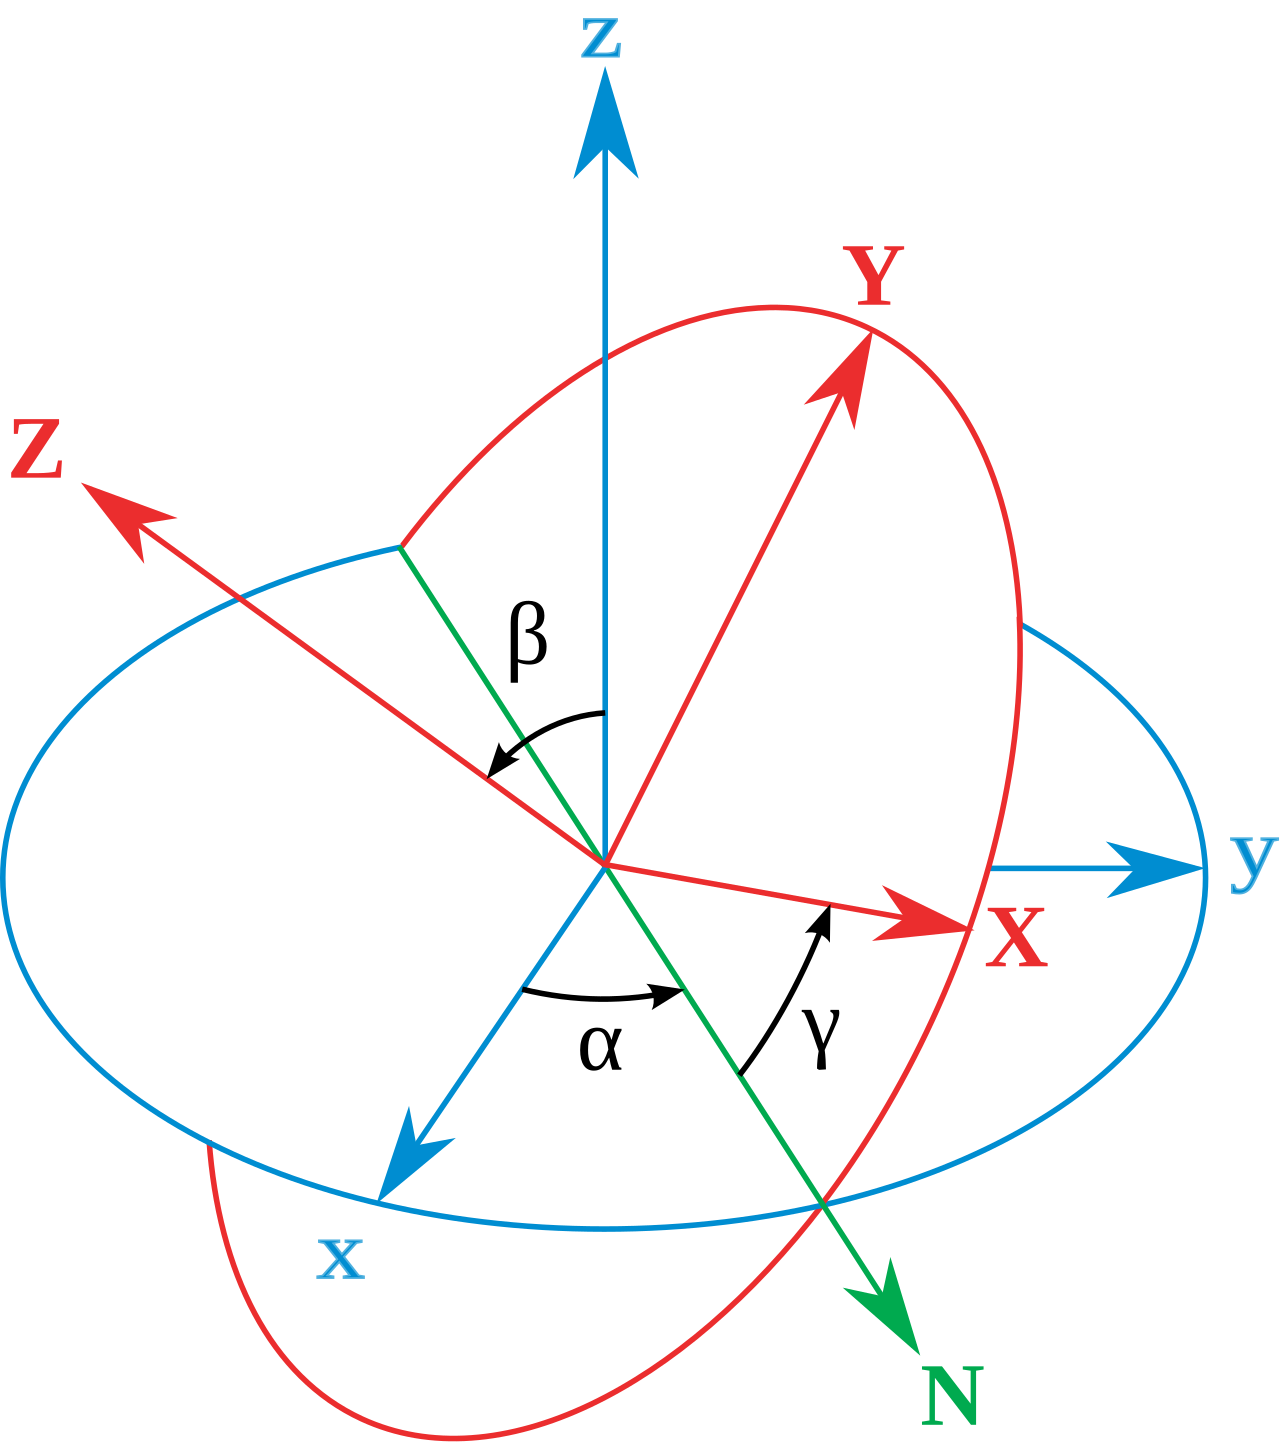
\includegraphics[width=0.65\textwidth]{Images/agent/he_toa_do_drone.png}
    \caption[Hệ tọa độ vật thể Body Frame của Quadcopter]{\bfseries\fontsize{12pt}{0pt}\selectfont Hệ tọa độ vật thể Body Frame của Quadcopter}
    \label{fig:he_toa_do_drone}
\end{figure}

Nguyên lý cân bằng và di chuyển của Quadcopter cấu hình Quad-X dựa trên chiều quay đối xứng của 4 motor (Hình \ref{fig:chieu_quay_motor}):
\begin{itemize}
    \item \textbf{Động cơ quay nghịch CCW}: Động cơ M1 (trước - phải) và M3 (sau - trái).
    \item \textbf{Động cơ quay thuận CW}: Động cơ M2 (sau - phải) và M4 (trước - trái).
\end{itemize}

\begin{figure}[H]
    \centering
    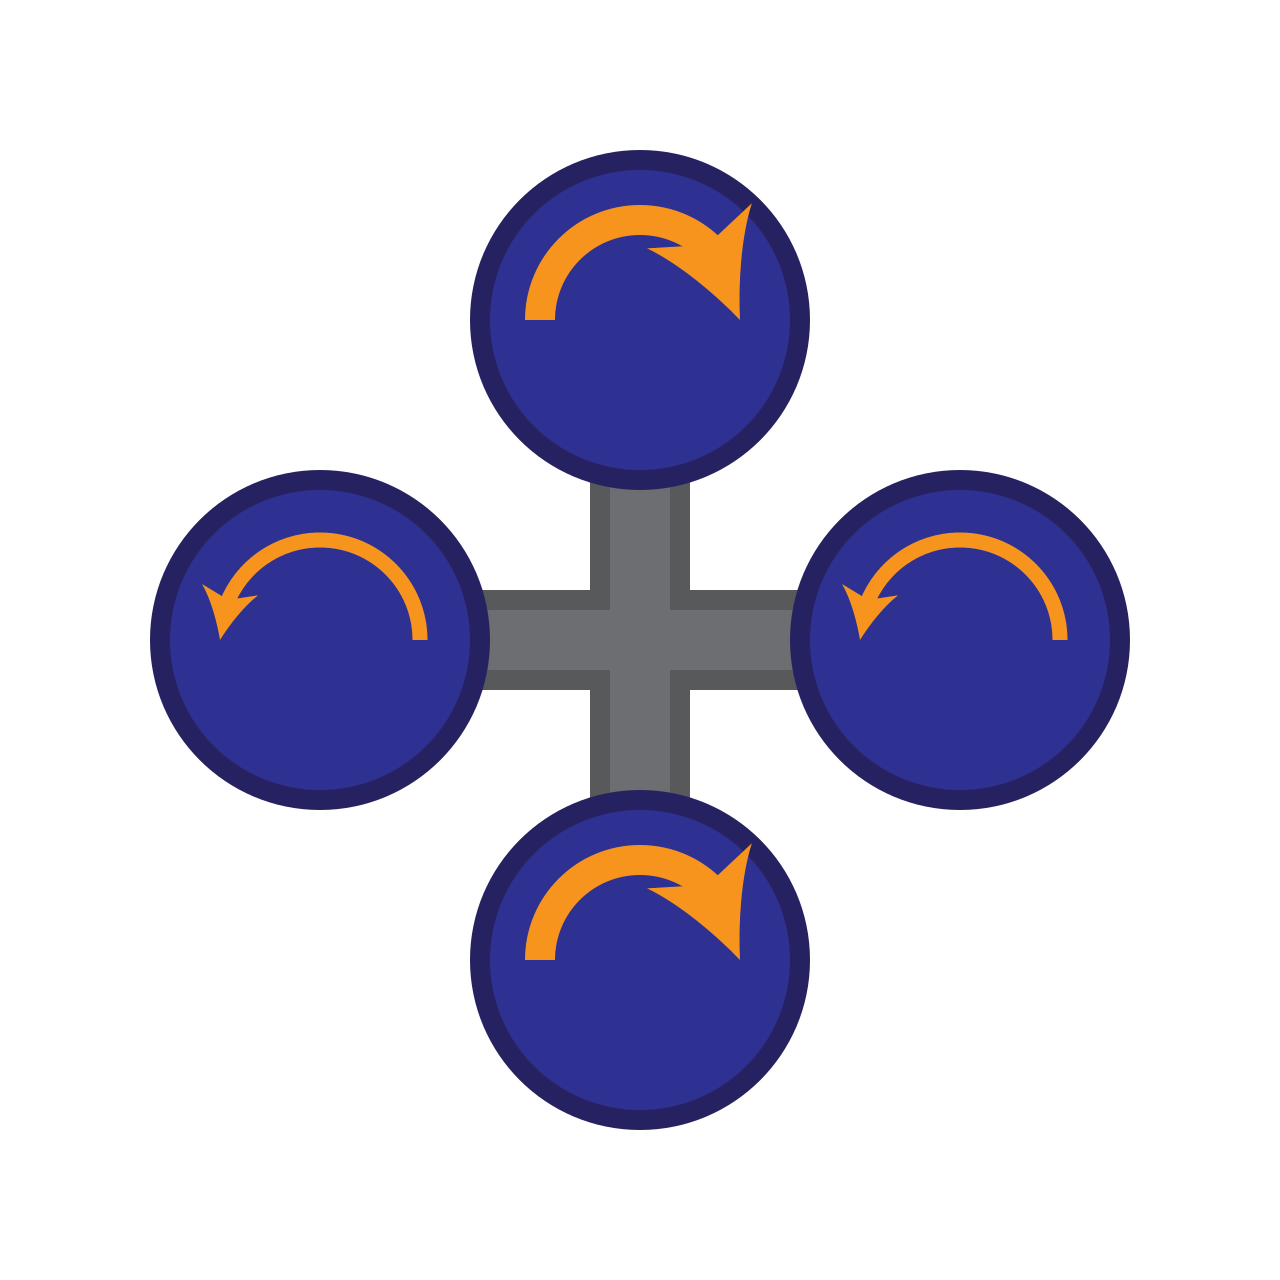
\includegraphics[width=0.65\textwidth]{Images/agent/chieu_quay_motor.png}
    \caption[Sơ đồ chiều quay động cơ cấu hình Quad-X]{\bfseries\fontsize{12pt}{0pt}\selectfont Sơ đồ chiều quay động cơ cấu hình Quad-X}
    \label{fig:chieu_quay_motor}
\end{figure}

Việc thay đổi tốc độ tương đối giữa các cặp động cơ tạo ra momen lực lệch thăng bằng để thực hiện các hành vi cơ động:
\begin{itemize}
    \item \textbf{Nghiêng phải (Roll dương)}: Tăng tốc các động cơ bên trái (M3, M4) và giảm tốc các động cơ bên phải (M1, M2).
    \item \textbf{Chúi mũi trước (Pitch âm)}: Tăng tốc các động cơ phía sau (M2, M3) và giảm tốc các động cơ phía trước (M1, M4).
    \item \textbf{Xoay trái CCW (Yaw dương)}: Tăng tốc các động cơ quay thuận CW (M2, M4) và giảm tốc các động cơ quay nghịch CCW (M1, M3). Mô-men phản lực lệch hướng sẽ làm thân drone xoay theo chiều ngược lại.
\end{itemize}

\subsection{Hệ thống điều khiển phản hồi PID vòng kín rời rạc}

Để duy trì sự cân bằng của Quadcopter trước các luồng gió nhiễu động từ môi trường bên ngoài, hệ thống nhúng liên tục chạy thuật toán điều khiển phản hồi PID vòng kín (Proportional-Integral-Derivative) trong miền rời rạc. Sơ đồ khối của bộ điều khiển được thể hiện trong Hình \ref{fig:so_do_khoi_pid}.

\begin{figure}[H]
    \centering
    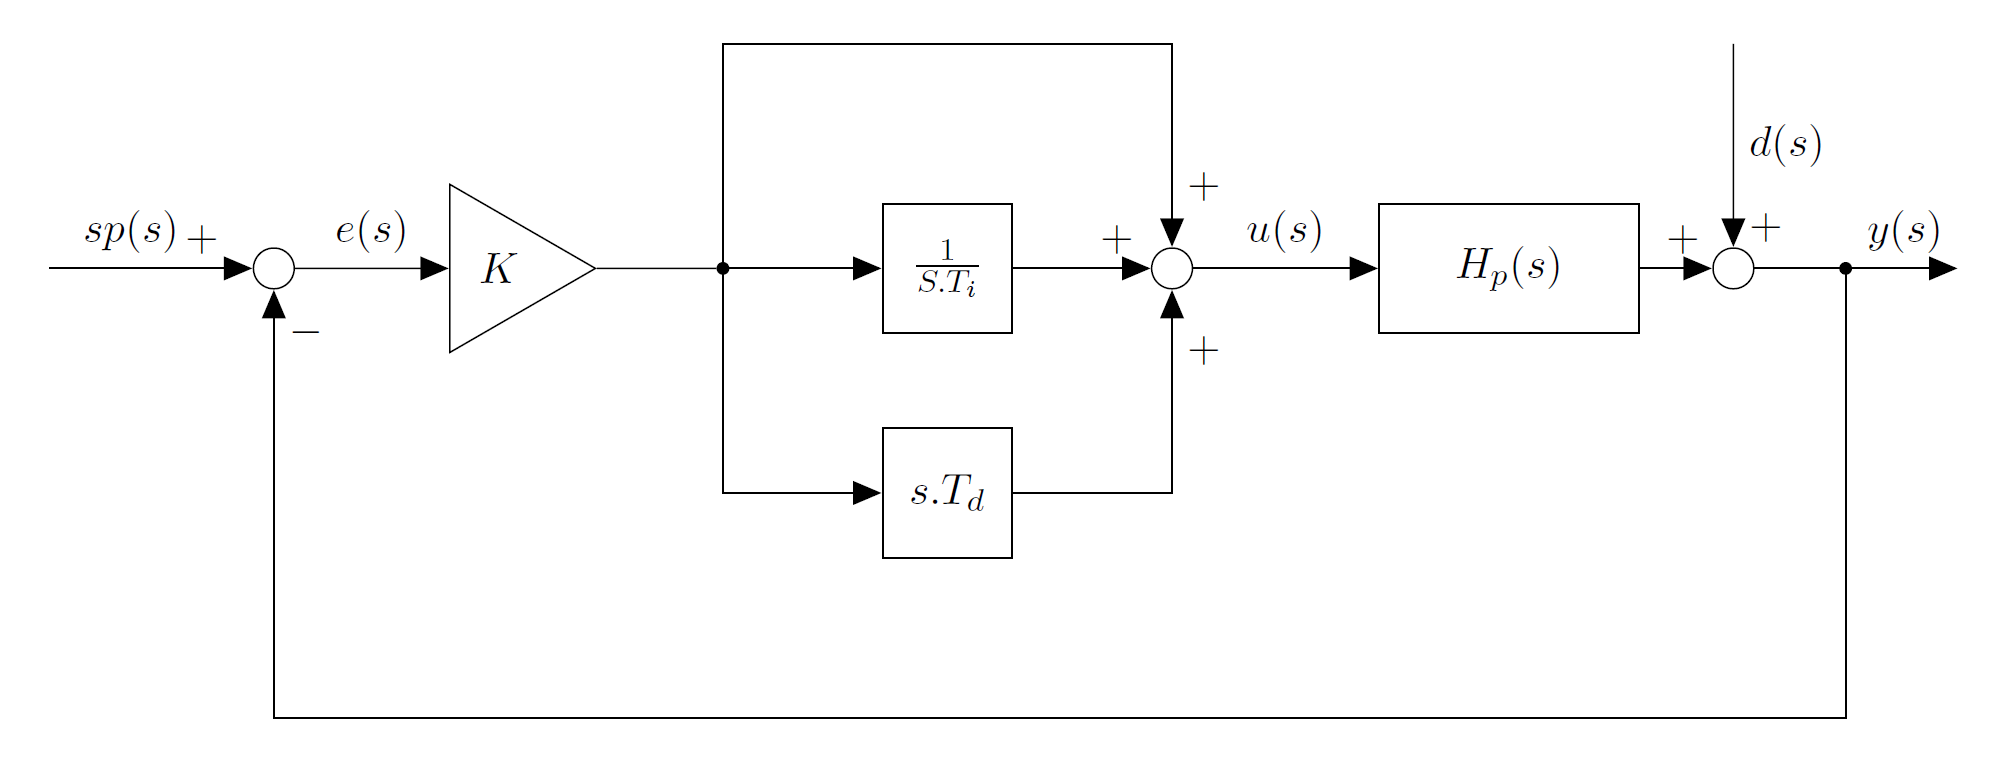
\includegraphics[width=0.85\textwidth]{Images/agent/so_do_khoi_pid.png}
    \caption[Sơ đồ khối bộ điều khiển phản hồi PID rời rạc]{\bfseries\fontsize{12pt}{0pt}\selectfont Sơ đồ khối bộ điều khiển phản hồi PID rời rạc}
    \label{fig:so_do_khoi_pid}
\end{figure}

Sai số góc nghiêng $e(t)$ tại thời điểm trích mẫu $n$ được định nghĩa bằng hiệu số giữa giá trị đặt từ tay điều khiển $Setpoint$ và góc nghiêng thực tế đo từ cảm biến $Feedback$:
\begin{equation}
    e[n] = Setpoint[n] - Feedback[n]
\end{equation}

Tín hiệu điều khiển đầu ra của khâu PID rời rạc được tính bằng công thức:
\begin{equation}
    u[n] = K_p \cdot e[n] + K_i \sum_{j=0}^{n} e[j] \cdot T + K_d \frac{e[n] - e[n-1]}{T}
\end{equation}
Trong đó, $T$ là chu kỳ trích mẫu của vòng điều khiển. Đối với hệ thống điều khiển nhúng Drone, hai hiện tượng kỹ thuật quan trọng cần được giải quyết triệt để trong firmware:

\begin{enumerate}
    \item \textbf{Hiện tượng bão hòa tích phân (Integral Windup)}: Xảy ra khi sai số lớn kéo dài khiến thành phần tích phân $I$ tăng quá mức giới hạn phần cứng của động cơ (vượt ngưỡng ga 2000$\mu s$). Khi Drone muốn đổi hướng gấp, khâu $I$ tích lũy quá lớn sẽ gây hiện tượng trễ đáp ứng nghiêm trọng, dẫn đến dao động quá đà hoặc lộn nhào (lật Drone). Thuật toán giải quyết bằng cơ chế **Anti-windup clamping** (khóa cứng giới hạn đầu ra khâu I ở mức $\pm 400$):
    \begin{equation}
        i\_mem = \max(\min(i\_mem + K_i \cdot e[n], PID\_MAX), -PID\_MAX)
    \end{equation}
    \item \textbf{Nhiễu khâu vi phân (Derivative Noise)}: Khâu vi phân cực kỳ nhạy cảm với các rung động cơ khí tần số cao của cánh quạt truyền qua khung sườn tới cảm biến IMU. Việc vi phân trực tiếp dữ liệu thô sẽ khuếch đại nhiễu làm nóng động cơ và gây cháy ESC. Hệ thống khắc phục bằng cách thiết lập **Bộ lọc thông thấp số IIR (Infinite Impulse Response)** bậc 1:
    \begin{equation}
        gyro\_input[n] = gyro\_input[n-1] \cdot 0.7 + new\_reading \cdot 0.3
    \end{equation}
\end{enumerate}

\subsection{Hệ thống cảm biến định vị quán tính IMU MPU6050 và Bộ lọc bù}

Cảm biến IMU MPU6050 \cite{mpu6050} tích hợp bộ cảm biến gia tốc 3 trục (Accelerometer) và cảm biến vận tốc góc 3 trục (Gyroscope) như mô tả trong Hình \ref{fig:truc_mpu6050}.

\begin{figure}[H]
    \centering
    
\includegraphics[width=0.45\textwidth]{Images/agent/truc_mpu6050.png}
    \caption[Sơ đồ các trục cảm biến trên chip MPU6050]{\bfseries\fontsize{12pt}{0pt}\selectfont Sơ đồ các trục cảm biến trên chip MPU6050}
    \label{fig:truc_mpu6050}
\end{figure}

Nguyên lý tính toán góc nghiêng từ cảm biến IMU có các đặc điểm đối nghịch:
\begin{itemize}
    \item \textbf{Gyroscope}: Tính góc bằng cách tích phân vận tốc góc theo thời gian: $\theta_{gyro} = \theta + \omega \cdot dt$. Khâu này phản hồi rất nhanh trước các chuyển động động học đột ngột, nhưng tích lũy sai số theo thời gian tạo ra hiện tượng trôi góc (Drift) do nhiễu offset DC của cảm biến.
    \item \textbf{Accelerometer}: Tính góc bằng công thức lượng giác dựa trên véc-tơ gia tốc trọng trường $g$:
    \begin{equation}
        \theta_{accel} = \arctan2(a_y, a_z) \cdot \frac{180}{\pi}
    \end{equation}
    Gia tốc trọng trường là mốc quy chiếu tuyệt đối nên góc tính từ accelerometer không bị trôi theo thời gian, nhưng nó cực kỳ nhạy cảm với các lực gia tốc động học của Drone lúc di chuyển và rung động cơ khí, gây nhiễu tức thời lớn.
\end{itemize}

Để dung hợp ưu điểm của hai cảm biến, hệ thống triển khai bộ lọc bù rời rạc (Complementary Filter) \cite{mahony2008} như sơ đồ trong Hình \ref{fig:bo_loc_bu}.

\begin{figure}[H]
    \centering
    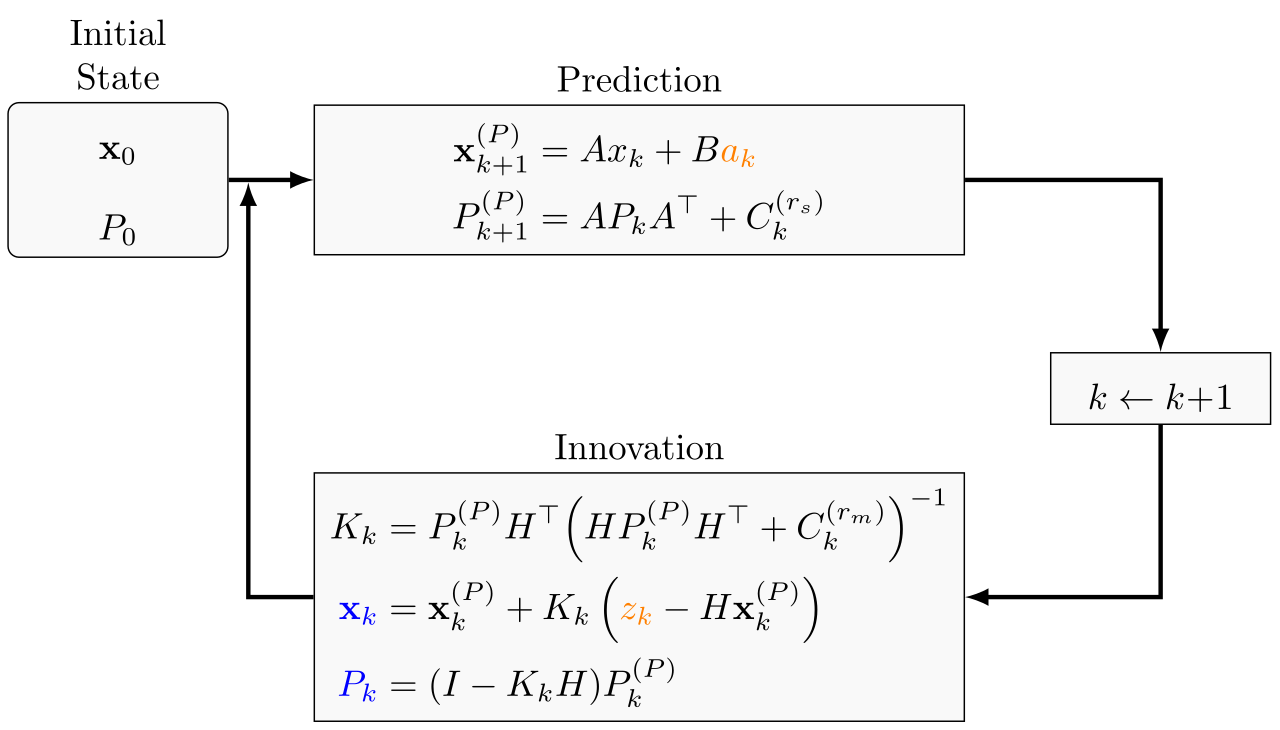
\includegraphics[width=0.8\textwidth]{Images/agent/bo_loc_bu.png}
    \caption[Sơ đồ thuật toán bộ lọc bù Complementary Filter]{\bfseries\fontsize{12pt}{0pt}\selectfont Sơ đồ thuật toán bộ lọc bù Complementary Filter}
    \label{fig:bo_loc_bu}
\end{figure}

Góc tư thế ước lượng tại mỗi chu kỳ trích mẫu được tính bằng công thức:
\begin{equation}
    \theta_{filter}[n] = \alpha \cdot (\theta_{filter}[n-1] + \omega_{gyro} \cdot dt) + (1 - \alpha) \cdot \theta_{accel}[n]
\end{equation}
Hệ số $\alpha$ được thiết lập bằng 0.98. Tỷ trọng này giúp hệ thống tin cậy 98\% vào sự thay đổi nhanh của Gyroscope trong thời gian ngắn, đồng thời liên tục lấy 2\% mốc tham chiếu tuyệt đối của Accelerometer để kéo góc lọc bù về giá trị thực, triệt tiêu hoàn toàn hiện tượng trôi góc.

\subsection{Giao thức truyền thông điều khiển vô tuyến CRSF và I2C}

ExpressLRS (ELRS) \cite{expresslrs2023} là công nghệ truyền sóng vô tuyến tầm xa mã nguồn mở hàng đầu hiện nay dựa trên công nghệ điều chế LoRa (Long Range), đem lại độ nhạy thu cực cao và khả năng xuyên nhiễu tuyệt đối. Bộ thu ELRS giao tiếp với Flight Controller thông qua giao thức truyền tin nối tiếp CRSF (Crossfire Protocol) với tốc độ baud rate tiêu chuẩn là 420.000\,bps.

Cấu trúc một khung dữ liệu CRSF được mô tả trực quan trong Hình \ref{fig:crsf_protocol}.

\begin{figure}[H]
    \centering
    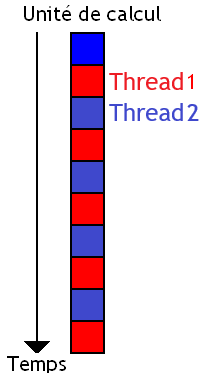
\includegraphics[width=0.85\textwidth]{Images/agent/crsf_protocol.png}
    \caption[Cấu trúc byte của khung dữ liệu giao thức CRSF]{\bfseries\fontsize{12pt}{0pt}\selectfont Cấu trúc byte của khung dữ liệu giao thức CRSF}
    \label{fig:crsf_protocol}
\end{figure}

Khung tin CRSF gồm các byte chức năng:
\begin{itemize}
    \item \textbf{Device Address (1 byte)}: Xác định đích đến (0xC8 cho Transmitter, 0xEE cho Flight Controller).
    \item \textbf{Frame Length (1 byte)}: Số lượng byte dữ liệu tiếp theo bao gồm cả byte CRC.
    \item \textbf{Type (1 byte)}: Định nghĩa loại dữ liệu (ví dụ 0x16 cho gói tin 16 kênh RC).
    \item \textbf{Payload (22 bytes)}: Chứa thông tin 16 kênh RC. Để tối ưu hóa băng thông, các kênh RC được đóng gói dưới dạng 11-bit trên mỗi kênh thay vì gửi 16-bit truyền thống.
    \item \textbf{CRC (1 byte)}: Mã kiểm tra lỗi CRC8 giúp loại bỏ hoàn toàn các khung tin bị sai lệch bit do nhiễu sóng.
\end{itemize}

Bên cạnh đó, việc lưu trữ các tham số cấu hình PID, căn chỉnh cảm biến được thực hiện qua bộ nhớ ROM EEPROM 24LC256 giao tiếp chuẩn I2C. Giản đồ xung timing của giao thức I2C được thể hiện trong Hình \ref{fig:i2c_timing}.

\begin{figure}[H]
    \centering
    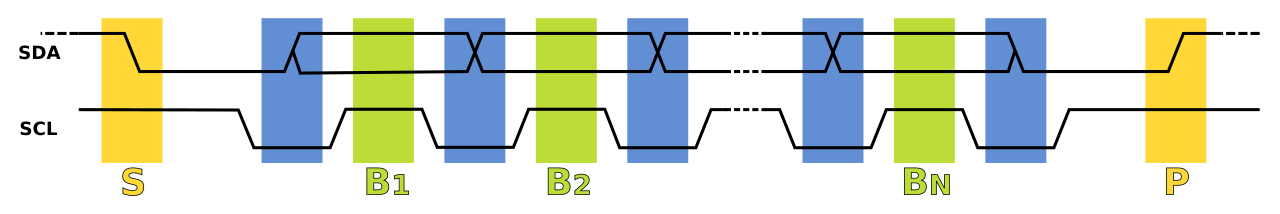
\includegraphics[width=0.85\textwidth]{Images/agent/i2c_timing.png}
    \caption[Giản đồ xung timing giao tiếp I2C giữa MCU và ngoại vi]{\bfseries\fontsize{12pt}{0pt}\selectfont Giản đồ xung timing giao tiếp I2C giữa MCU và ngoại vi}
    \label{fig:i2c_timing}
\end{figure}

Giao tiếp I2C sử dụng hai đường tín hiệu SCL (Serial Clock) và SDA (Serial Data). Cơ chế bao gồm xung START (SDA chuyển mức cao xuống thấp khi SCL cao), chuỗi bit dữ liệu đồng bộ theo nhịp clock SCL, bit ACK kiểm tra từ slave và xung STOP (SDA chuyển thấp lên cao khi SCL cao), giúp MCU ghi nhận cấu hình một cách chính xác tuyệt đối.
